\section{Implementation evidence and controlled comparisons}
\label{sec:experiments}

\subsection{Verification scope}

The integrated implementation passes 728 unit tests, with three skips for
unavailable optional dependencies, in the recorded Python 3.12.14
environment. The run includes all 31 newly added tests: ten for exact
quaternion and presentation compilation, thirteen for first jets and
continued rank-decision scans, and eight for streaming responses.
After the full run, an additional general-presentation API boundary was
tightened so callers cannot request the meridional shortcut without
validated diagram construction; the ten SU(2) tests were rerun and passed,
including a same-trace cyclic counterexample. The final archive retains
the logs and source manifest rather than relying on a test count in a
historical README.

The test oracles are intentionally different computations. Streaming
responses are compared with integer Bareiss cofactors from independently
reconstructed complete graphs. First-jet decisions are compared with
an independent full crossing cube, as well as the maintained exact scanner.
Representation queries are compared with a separate reduced Khovanov cube
and finite-group homomorphism counts. These checks test implementation
behavior on finite inputs; the theorems establish the universal statements.

\begin{center}\small
\begin{tabularx}{\textwidth}{@{}p{0.25\textwidth}YY@{}}
\toprule
Recorded check & Coverage & Result and qualification\\
\midrule
Integrated test suite & 728 tests, including 31 new tests & Passed; three optional-dependency skips.\\
First-jet discovery & 360 scans, 2898 stages; 117 eligible components & All pre/post-elimination profiles agree; all observed $t=\kappa$.\\
First-jet independent cube & 96 comparisons on 32 sampled knots & No decision disagreement; continued replacements and budget fallback included.\\
Streaming integer oracle & 53 diagrams, 610 suffixes, 19520 comparisons & No mismatch; singular and characteristic-two cases included.\\
SU(2) short-budget audit & 96 queries on 48 sampled entries, 38 distinct PD arrays & 90 complete and correct, six inconclusive.\\
Finite-group presentation audit & 36 sampled entries, 26 distinct PD arrays & Equal $S_3$ homomorphism counts for all three presentations.\\
\bottomrule
\end{tabularx}\end{center}

\subsection{First-jet observer: eligibility and timing are different results}

The discovery experiment in Section~\ref{sec:first-jet-pre-schur} establishes
that the pre-elimination test encounters eligible components in actual
diagrams. Its 117 components contain 633 objects and 237 scalar pairs.
All contain scalar units, so they lie outside the old radical-only
observer's precondition at that moment. This does not by itself imply a
speedup: traversing the whole graph and computing ranks also costs work.

The paired benchmark therefore compares six raw-scanner arms on twelve
actual diagrams: the ordinary scanner, an identical control, the full
first-jet scanner, an observe-only variant, a variant without completion
geometry, and a zero-observation-budget fallback. Every arm validates the
same supplied PD and uses the same crossing order, no shape cache, a
three-second deadline and a 50,000-object ceiling. Timings include validation,
scanner construction, observation, and elimination. They exclude imports,
input construction, order selection, and one warmup. Front-end recognizer
filters are bypassed. Seven shuffled rounds are recorded; small cases
batch repeated calls as specified by the script. All arms finish in every
recorded case.

\begin{table}[htbp]
\centering\small
\begin{tabular}{@{}lrrrrrr@{}}
\toprule
Input & $n$ & Standard ms & Jet ms & Paired ratio & A/A & Repl.\\
\midrule
Trefoil & 3 & 0.336 & 0.364 & 0.922 & 0.954 & 0\\
Conway & 11 & 3.362 & 4.605 & 0.795 & 1.009 & 0\\
Kinoshita--Terasaka & 11 & 4.625 & 6.410 & 0.761 & 1.018 & 0\\
Hard unknot fixture & 8 & 0.780 & 0.840 & 0.893 & 1.065 & 0\\
Scrambled grid unknot & 6 & 0.363 & 0.682 & 0.525 & 1.033 & 3\\
Five-strand stress braid & 36 & 301.156 & 483.852 & 0.663 & 0.964 & 0\\
Conway connected sum & 22 & 52.323 & 15.007 & 3.367 & 1.009 & 0\\
Coxeter unknot & 11 & 0.334 & 1.077 & 0.310 & 0.989 & 10\\
Coxeter unknot & 35 & 1.147 & 5.864 & 0.192 & 0.895 & 34\\
Trefoil with 8 cancelling pairs & 19 & 1.795 & 2.110 & 0.848 & 1.015 & 0\\
Trefoil with 24 cancelling pairs & 51 & 4.569 & 5.651 & 0.750 & 1.008 & 0\\
$T(3,5)$ & 10 & 2.440 & 2.702 & 0.895 & 0.988 & 0\\
\bottomrule
\end{tabular}
\caption{All twelve first-jet benchmark cases. Times are medians;
``paired ratio'' is the median of the seven within-round
standard/jet ratios and therefore need not equal the ratio of the two
displayed medians. A/A is the corresponding standard/control statistic.
Repl. counts installed multiplier-one replacements. Ratios below one
mean the first-jet arm is slower.}
\label{tab:jet-timings}
\end{table}

The clear gain is the connected sum of two Conway diagrams. At crossing
11 of 22 it has a 975-object whole one-matching block with scalar rank
471 and $t=\kappa=33$. The actual matching completion is a knot, so the
rank lower bound is 66 and the scan rejects immediately. Counted
cobordism compositions fall from 3324 to 39. No replacement occurs.
The observe-only arm has paired ratio 3.473, confirming that the gain is
early rejection. Disabling completion geometry removes this certificate
and has ratio 0.569.

The three cases that actually install replacements are slower, with
ratios 0.525, 0.310, and 0.192. Their ordinary scans already perform
zero counted cobordism compositions, so there is little expensive work
for the first-jet query to avoid. The remaining full-jet ratios range
from about 0.663 to 0.922. These unfavorable results are consequential:
the implementation is useful as an exact experimental interface, but
the data do not justify a default global replacement policy. The
Conway-sum case is also decomposable and does not establish a whole-pipeline
improvement over the repository's existing structural reductions.

\begin{figure}[htbp]
\centering
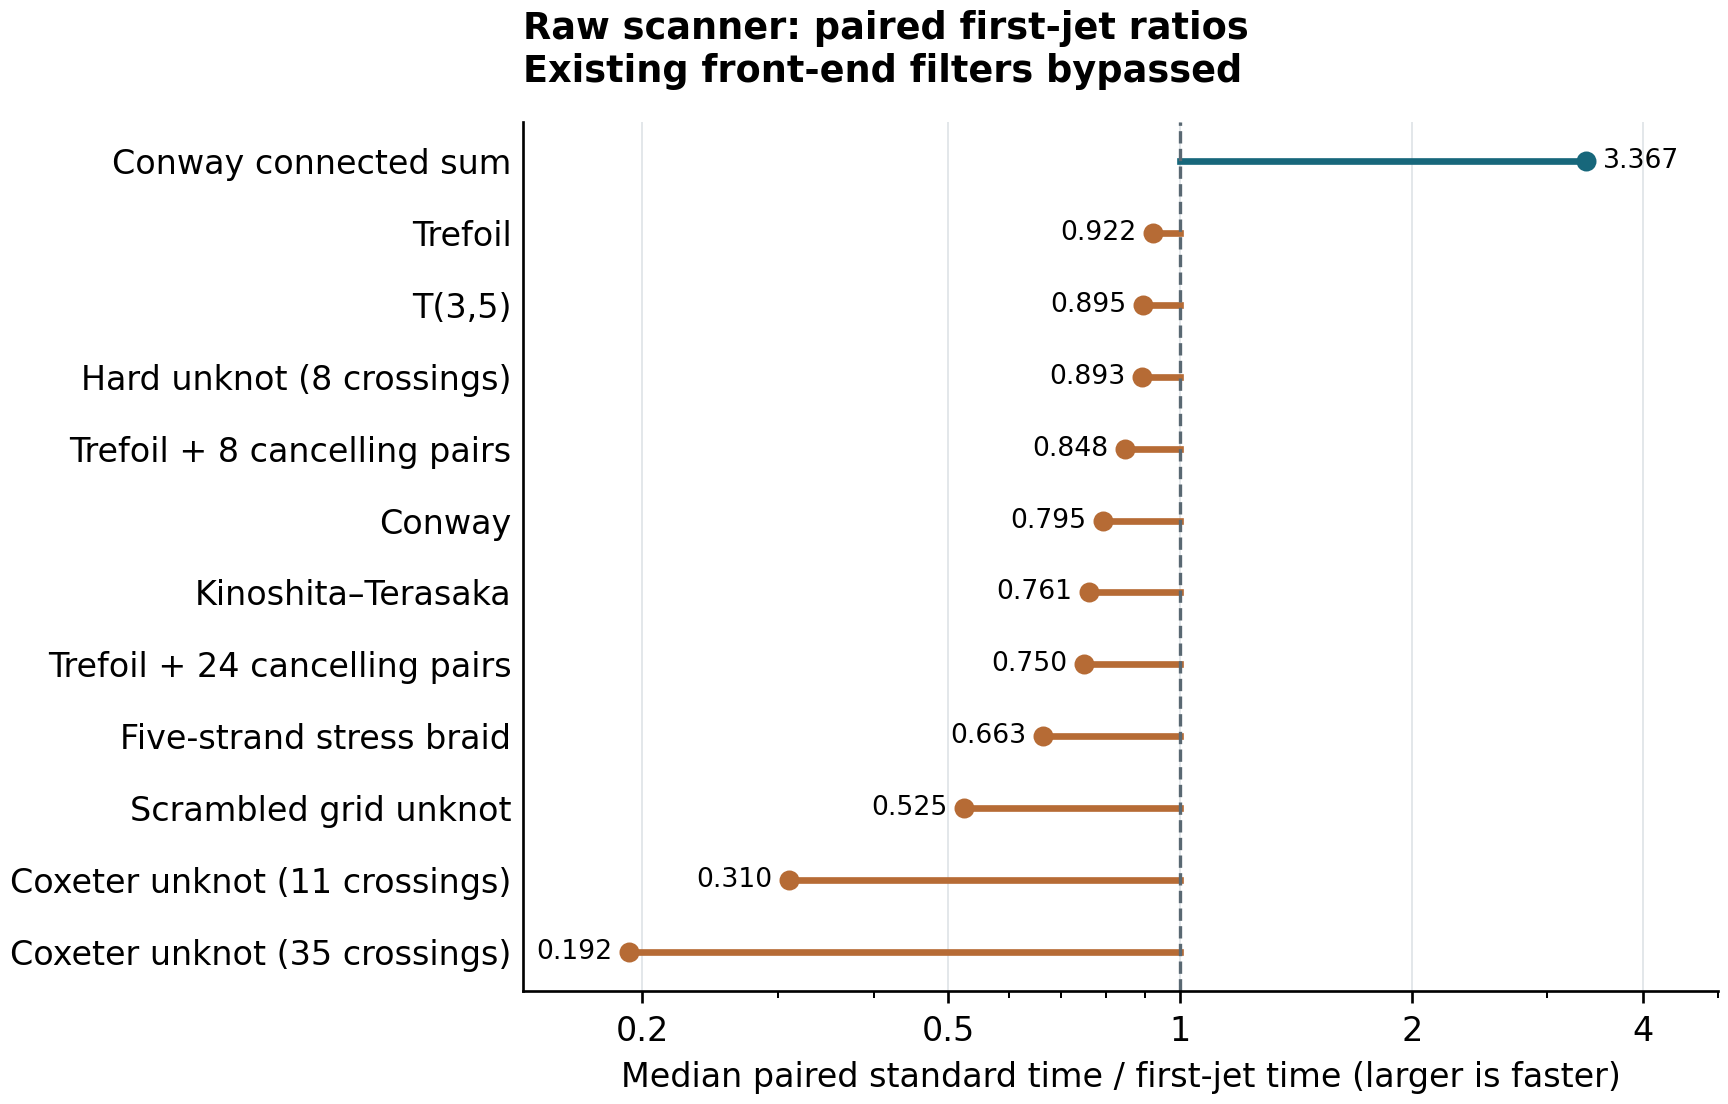
\includegraphics[width=\textwidth]{figures/first_jet_ratios.png}
\caption{All first-jet paired ratios from Table~\ref{tab:jet-timings}.
The dashed line is equal runtime. The early Conway-sum obstruction is
the only improvement in this raw-scanner corpus; replacement cases regress.}
\label{fig:jet-ratios}
\end{figure}

% Derived only from the existing su2_audit.json and su2_benchmark.json.
% No experiments were rerun for this subsection.

\subsection{SU(2) compilation and decision experiments}
\label{subsec:su2-experiments}

The recorded experiments test the exact formula construction and illustrate
the practical degree--variable tradeoff with the exact NLSAT method\cite{JovanovicDeMoura2012,ProgrammingZ3}.  They do not measure the running
time of the theoretical real-decision algorithm.  The complete records are
\path{results/su2_audit.json} and
\path{results/su2_benchmark.json}; the corresponding scripts are
\path{su2_research/audit_su2.py} and
\path{su2_research/benchmark_su2.py}.

\paragraph{Finite correctness audit.}
With seed $20261008$, the audit sampled 48 accepted one-component braid
closures on two to four strands, using words of one to seven letters.
Every third accepted diagram was mirrored.  An independently implemented
reduced $\mathbb F_2$ Khovanov cube classified 39 samples as unknots
and nine as knotted.  Bridge compilation completed 42 of 48 queries:
36 unknot decisions and six knottedness decisions.  Its six timeouts
comprised three samples of each oracle class.  Defining-generator Tietze
elimination followed by compilation completed all 48 queries.  Thus 90 of
96 queries were definitive, with no disagreement among those 90.
The audit identifies its exact backend as Z3 5.1.0.

These are 48 sampled entries, containing 38 distinct stored PD arrays,
and do not constitute 48 distinct knot types or an independent test-set
estimate of general success probability.  The saved PD arrays specify
the actual inputs: the stored source braid words precede the optional
mirroring step.  The seed and script reproduce that step.
For the 36 sampled entries with at most five crossings, comprising 26
distinct PD arrays, exhaustive counts of homomorphisms to $S_3$ agreed
for the Wirtinger, bridge, and simplified presentations.  This checks
concrete relation-order and substitution behavior; agreement for one
finite target group does not establish presentation equivalence in
general.  The Tietze and bridge proofs supply that justification.

The same audit checked the prime-pretzel family at
$m=3,5,7,11,21,51$, hence at $9,15,21,33,63,153$ crossings.
The computed Fox $3$-coloring dimensions were respectively
$3,5,7,11,21,51$, as predicted by
Proposition~\ref{prop:su2-prime-rank-obstruction}.  These finite checks
support the construction and indexing; the proposition's proof supplies
the statement for all odd $m$.

\paragraph{Presentation choice and peak degree.}
The benchmark makes three repetitions per presentation on seven fixed
examples, with a requested solver allowance of $250$ milliseconds.
Table~\ref{tab:su2-recorded-bench} reports representative cases.
Here $k$ is the actual number of real variables after the safe gauge and
meridional trace sharing, and $d_{\rm eq}$ is the maximum degree of an
individual compiled equality before squaring.  The implementation sends
the separate equations to NLSAT in these measurements.  Its sum-of-squares
aggregate is available separately for the constant-atom theoretical bound.

\begin{table}[htbp]
\centering
\small
\begin{tabular}{llrrrrl}
\hline
Input & Presentation & $k$ & $d_{\rm eq}$ & Compile ms & Query ms & Result\\
\hline
Figure-eight & Wirtinger & 10 & 4 & 0.702 & 273.510 & I\\
 & Bridge & 10 & 2 & 0.416 & 270.820 & I\\
 & Tietze & 4 & 10 & 1.716 & 26.103 & K\\
$T(2,9)$ & Wirtinger & 25 & 4 & 1.866 & 283.346 & I\\
 & Bridge & 25 & 2 & 0.972 & 285.034 & I\\
 & Tietze & 4 & 18 & 11.411 & 72.254 & K\\
Coxeter unknot, $n=9$ & Wirtinger & 25 & 4 & 1.519 & 280.035 & I\\
 & Bridge & 2 & 2 & 0.323 & 0.983 & U\\
 & Tietze & 2 & 2 & 0.319 & 1.232 & U\\
\hline
\end{tabular}
\caption{Recorded medians of three repetitions, in milliseconds.  K:
nonabelian representation; U: no nonabelian representation; I:
inconclusive timeout.  All three repetitions in each row had the displayed
status.  The Coxeter example is the closure of
$\sigma_1\cdots\sigma_9\in B_{10}$.  Timeout durations are reported
as censored runs and are not completion times.}
\label{tab:su2-recorded-bench}
\end{table}

On $T(2,9)$, Tietze elimination reduced $k$ from 25 to four while
raising $d_{\rm eq}$ to 18, with aggregate degree bound 36.
Its compilation took longer, but its query completed within the requested
allowance while the other two formulations did not.  This demonstrates
why generator elimination must be assessed together with degree and
support growth.  It gives no finite speedup ratio against a censored run.
Across all 63 benchmark queries, 39 were definitive and 24 inconclusive.

\paragraph{Compressed powers.}
A separate construction-only experiment uses the general presentation
$\langle x_1,x_2\mid x_1^{2^b}\rangle$, represented by $b$ squaring
gates.  It has no knot-group provenance and was not assigned a knot
verdict.  Table~\ref{tab:su2-recorded-powers} shows that the compiler
retained the circuit, producing constant-degree equations without
expanding $2^b$ letters.  The number of stored terms sums the supports
of the individual equations and the nonabelian polynomial; it is not the
support of a fully collected sum-of-squares aggregate.

\begin{table}[htbp]
\centering
\small
\begin{tabular}{rrrrr}
\hline
$b$ & Real variables & Stored terms & $d_{\rm eq}$ & Compile ms\\
\hline
8 & 37 & 97 & 2 & 0.260\\
32 & 133 & 361 & 2 & 0.815\\
128 & 517 & 1417 & 2 & 3.160\\
512 & 2053 & 5641 & 2 & 13.622\\
2048 & 8197 & 22537 & 2 & 54.236\\
\hline
\end{tabular}
\caption{Three-run compiler medians for an already constructed word
circuit.  Expanded word length is $2^b$; aggregate degree bound is four
throughout.  These measurements exclude WordArena construction and make
no claim about solver performance on the resulting formulas.}
\label{tab:su2-recorded-powers}
\end{table}

\paragraph{Interpretation and trust boundary.}
Both scripts enable a trace-zero witness probe before the unrestricted
query. A satisfying assignment to this restricted query is valid for
the original formula; an unsatisfiable or unknown probe is discarded by
this implementation. The known completeness theorem for verified knot
meridians, Theorem~\ref{thm:su2-traceless}, would permit a stronger
knot-specific policy, but these recorded runs do not implement it.
All 15 successful knottedness queries in the audit used this probe.
Their exact algebraic model expressions were retained and checked against
the assertions by Z3 itself.  This remains a trusted-solver computation,
not an independently checked proof certificate.  Neither a trace-zero
failure nor any timeout is accepted as an unknot decision.

The timing allowances are soft: the largest recorded audit call took
$375.926$ milliseconds with a requested $300$-millisecond allowance,
and the largest benchmark query took $288.326$ milliseconds with a
requested $250$-millisecond allowance.  The benchmark's reported query
time includes formula parsing and solver checks, but excludes the Z3
import and subsequent model extraction and validation.  Its compiler
times exclude construction of the input diagram.  The audit's per-call
times cover compilation and the solver wrapper.

The identical repeated compiler controls also show appreciable timing
variation: across 63 pairs, the median first-run/control ratio was 1.234,
with range 0.609--5.565.  Since the control always runs second, this
includes order and warm-up effects.  With three repetitions, fixed case
order, and a small convenience sample, the data justify neither a
statistical speedup claim nor an extrapolated asymptotic exponent.
They document correct completed queries and concrete representation
tradeoffs.  Renegar's theoretical complexity and this optional NLSAT
implementation remain separate statements.


\subsection{Interpreting the response measurements}

Section~\ref{sec:streaming-response} reports the complete all-suffix setup
experiment because its arithmetic and geometry scopes belong together.
At 256 crossings, dense rebuilding takes 3615.101 ms and streaming takes
14.061 ms, a recorded ratio of 257.10; the identical dense control ratio
is 0.906. The new arithmetic theorem, the reduction from 23,789,518 to
928 elimination updates, and the small carried matrices explain the
direction of the gain without depending on an exact wall-clock ratio.

The input family is easy for the recognition front end. The streaming-only
8192-crossing run demonstrates capacity for many evolving suffixes,
not difficulty of those knot types. A future integration experiment
must retain inputs on which the recognizer actually demands many such
responses, and include the setup cost even if an early certificate
ends the scan. The present release therefore makes no default-recognizer
speedup claim from this experiment.

\begin{figure}[htbp]
\centering
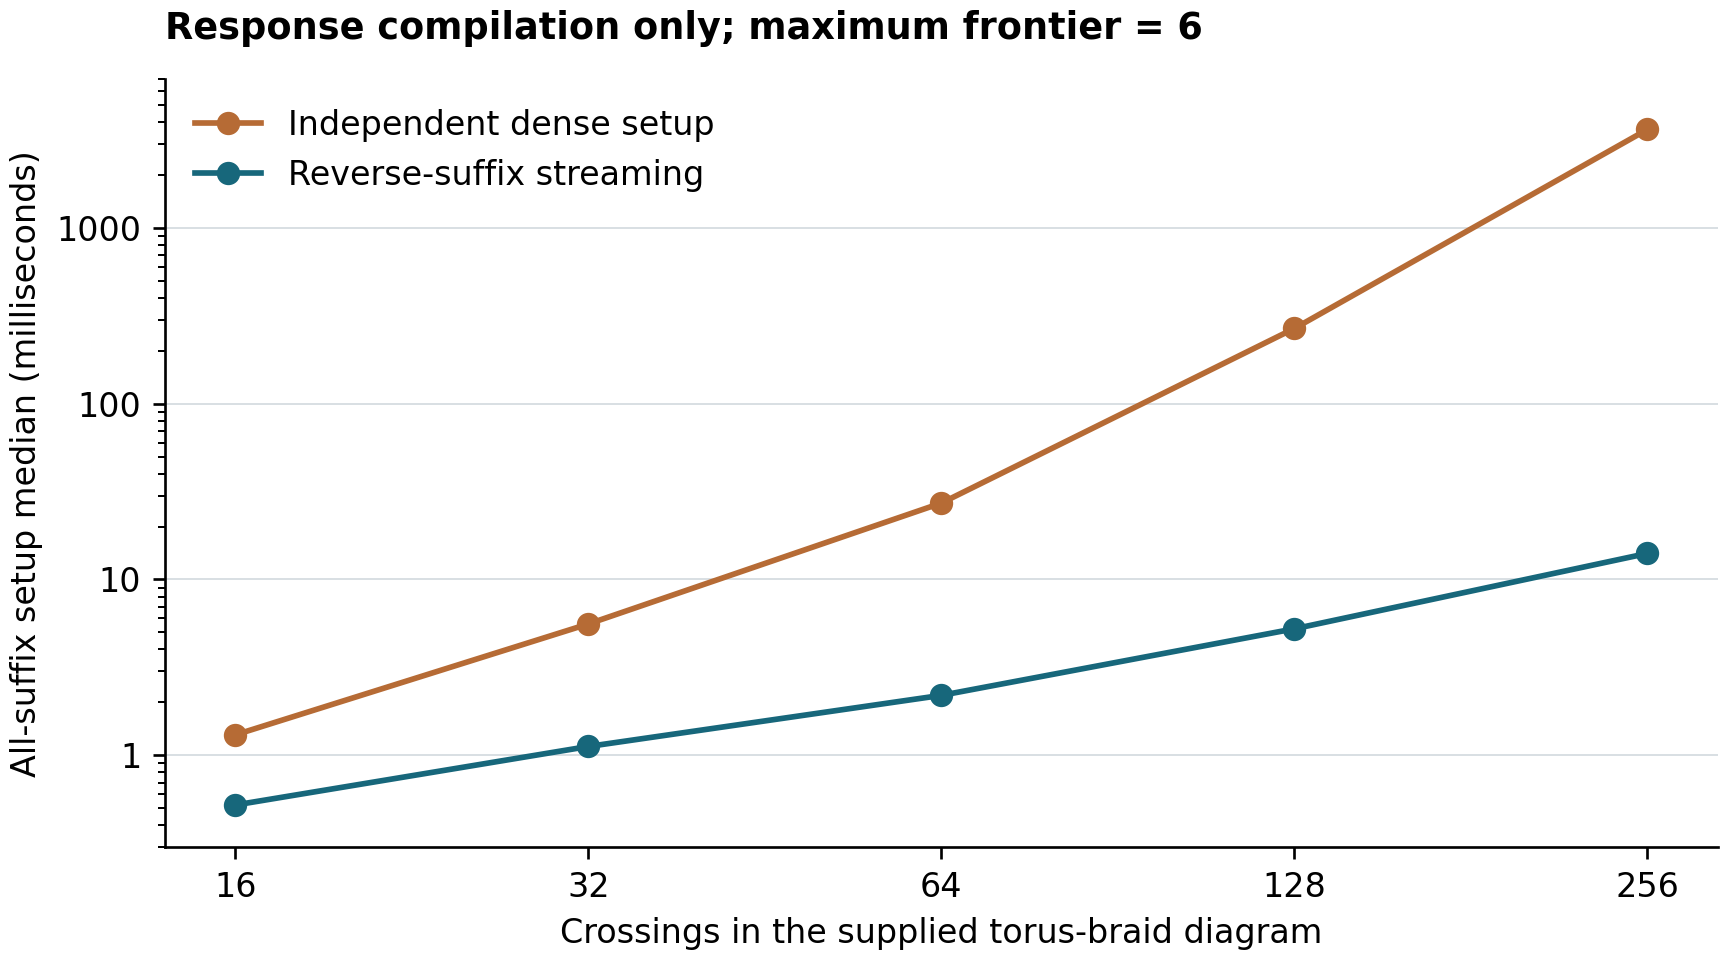
\includegraphics[width=\textwidth]{figures/response_setup.png}
\caption{Recorded all-suffix setup medians at frontier six, with logarithmic
axes. These are easy torus-braid inputs and subroutine timings. The plot
shows the recorded points only; it does not fit an asymptotic exponent.}
\label{fig:response-setup}
\end{figure}

\subsection{What these experiments do not establish}

No finite corpus establishes universal checkpoint bounds, small
presentations, or a success probability on arbitrary knots. No timeout is
counted as an exact answer or as a completed baseline runtime. No
exponent is estimated from the timing table. No synthetic word circuit
is promoted to a knot input without group provenance. The tests and
measurements support implementation claims and identify costs worth
reducing; the asymptotic claims come from the explicit proofs.
